\documentclass[10pt, landscape]{article}
\usepackage[scaled=0.92]{helvet}
\usepackage{multicol}
\usepackage{calc}
\usepackage{ifthen}
%\usepackage[landscape]{geometry}
\usepackage[a4paper,margin=3mm,landscape]{geometry}
% Standardised 3mm margins


\usepackage{newtxtext} 

%for strikeout
\usepackage{ulem}

%For editing parbox
\usepackage[table]{xcolor}
%For editing itemise margins, reduce iterm separaion and list separation
\usepackage{enumitem}

% For math -------------------
\usepackage{amsmath,amsthm,amsfonts,amssymb}
\usepackage{mathtools}
%  convenient absolute value symbol
\newcommand{\abs}[1]{\vert #1 \vert}
%  convenient floor and ceiling
\newcommand{\floor}[1]{\lfloor #1 \rfloor}
\newcommand{\ceil}[1]{\lceil #1 \rceil}
%  convenient modulo
\newcommand{\Mod}[1]{\ \mathrm{mod}\ #1}
%  for logical not operator, iff symbol, convenient "if/then"
\renewcommand{\lnot}{\mathord{\sim}}
\let\then\rightarrow
\let\Then\Rightarrow
%  vectors
\newcommand{\vv}[1]{\boldsymbol{#1}}
\newcommand{\VV}[1]{\overrightarrow{#1}}
%  column vector
\newcommand{\cvv}[1]{\left(\begin{smallmatrix}#1\end{smallmatrix}\right)}
%\newcommand{\code}[1]{\textcolor{myblue}{\texttt{#1}}}
\newcommand\bggreen{\cellcolor{green!10}}
\makeatother
\definecolor{myblue}{cmyk}{1,.72,0,.38}
\everymath\expandafter{\the\everymath \color{myblue}}
% --------------------------


%For pictures / figures
\usepackage{color,graphicx,overpic}
\graphicspath{ {./images/} }

%\usepackage{newtxtext} 
%\usepackage{amssymb}
%\usepackage[table]{xcolor}
%\usepackage{vwcol}
%\usepackage{tikz}
%\usepackage{wrapfig}
%\usepackage{makecell}


% For Code Blocks
\usepackage{xcolor}
\usepackage{listings}

\lstdefinestyle{mystyle}{
	backgroundcolor=\color{gray!25!white},
	basicstyle=\scriptsize,
	numbers=none,    %or = none or left
	showstringspaces=false,
	breaklines=true,
	breakatwhitespace=false,                  
	captionpos=b,                    
	keepspaces=true,                                 
	numbersep=5pt,                  
	showspaces=false,                
	showtabs=false,                  
	tabsize=2,
 }
%Helpful:
%[linewidth = 1.0 \linewidth]
%\lstinline{}
% use \code{} for \lstinline with colorbox.
\newcommand{\code}[1]{\colorbox{gray!25!}{\lstinline|#1|}}
\lstset{style=mystyle}



%--------------------------- PACKAGES ABOVE --------------------------------------------------------------

\pdfinfo{
  /Title (CS2040S.pdf)
  /Creator (Ger Teck)
  /Author (Ger Teck)
  /Subject ()
  /Keywords (tex)}

% Turn off header and footer
\pagestyle{empty}

% for tight centres (less spacing)
\newenvironment{tightcenter}{%
  \setlength\topsep{0pt}
  \setlength\parskip{0pt}
  \begin{center}
}{%
  \end{center}
}

% Redefine section commands to use less space
\makeatletter
\renewcommand{\section}{\@startsection{section}{1}{0mm}%
                                {-1ex plus -.5ex minus -.2ex}%
                                {0.5ex plus .2ex}%x
                                {\normalfont\large\bfseries}}
\renewcommand{\subsection}{\@startsection{subsection}{2}{0.1mm}%
                                {-1explus -.5ex minus -.2ex}%
                                {0.5ex plus .2ex}%
                                {\normalfont\normalsize\bfseries}}
\renewcommand{\subsubsection}{\@startsection{subsubsection}{3}{0.1mm}%
                                {-1ex plus -.5ex minus -.2ex}%
                                {1ex plus .2ex}%
                                {\normalfont\small\bfseries}}
% change font
%\renewcommand{\familydefault}{\sfdefault}
%\renewcommand\rmdefault{\sfdefault}
\linespread{1.05}

\makeatother

% Define BibTeX command
\def\BibTeX{{\rm B\kern-.05em{\sc i\kern-.025em b}\kern-.08em
    T\kern-.1667em\lower.7ex\hbox{E}\kern-.125emX}}

% Don't print section numbers
\setcounter{secnumdepth}{0}

\setlength{\parindent}{0pt}
\setlength{\parskip}{0pt plus 0.5ex}

\setlength{\parindent}{0pt}
\setlength{\parskip}{0pt plus 0.5ex}
%% this changes all items (enumerate and itemize)
\setlength{\leftmargini}{0.5cm}
\setlength{\leftmarginii}{0.4cm}
\setlength{\leftmarginiii}{0.5cm}
\setlist[itemize,1]{leftmargin=2mm,labelindent=1mm,labelsep=1mm}
\setlist[itemize,2]{leftmargin=3mm,labelindent=1mm,labelsep=1mm}
\setlist[itemize,3]{leftmargin=3mm,labelindent=1mm,labelsep=1mm}
%itemsep = 0mm
\setlist{nosep}

% Need Logo Picture
%Watermark Top Right
%\usepackage{atbegshi,picture}
%\AtBeginShipout{\AtBeginShipoutUpperLeft{%
 % \put(\dimexpr\paperwidth-1.2cm\relax, -1.2cm){\makebox[0pt][r]{\framebox{
\includegraphics[width = 0.3cm]{mountainbooks} Ger Teck}}}%
%}}


% -------------------------------------------------------------------------------

% START OF DOCUMENT HERE

\begin{document}
\raggedright
\footnotesize
\begin{multicols}{4}



% multicol parameters
% These lengths are set only within the two main columns
\setlength{\columnseprule}{0.25pt}
\setlength{\premulticols}{1pt}
\setlength{\postmulticols}{1pt}
\setlength{\multicolsep}{1pt}
\setlength{\columnsep}{2pt}




% TABLE PACKAGE 
 \begin{center}
    \fbox{%
        \parbox{0.8\linewidth}{\centering \textcolor{black}{
           \\ \normalsize{\textbf{CS2040S Midterm Summary}}
            \\ \normalsize{AY22/23 Sem 2}}
            \\ {\footnotesize github.com/gerteck}
            \\ {\footnotesize Adapted from github.com/jovyntls/cheatsheets/}
        }%
    }
  \end{center}
  
\section{Data Structures and Algorithms}
 \begin{itemize}
	\item Algorithm: finite sequence of steps, unambiguous and precise, to accomplish some task.
	\item \textbf{Desirable Traits} of algorithms: fast, efficient, fair, small memory, parallel, modular, correct, secure. Compare trade-offs
	\item \textbf{Midterms Key Topics}: Asymptotic Notation, Simple Recurrences, Asymptomatic Analysis, Basic Probability. 
	\item \textbf{Key Algorithms}: Binary search, Sorting, Balanced Binary Trees, Augmented Trees, Heaps. 
	\item \textbf{Key Ideas}: Problem Solving: Identify Invariants (to understand and show how algorithm works), Trade-offs (Choosing), Augmentation of data structures. 
	\item \textbf{Strategies:} Try something simple (Naive), Reduce and conquer (binary search), Divide and conquer (Mergesort), Maintaining invariant (AVL trees, keep sorted), Augment existing structure.
\end{itemize}


\section{ORDERS OF GROWTH}
\begin{itemize}
	\item Notations: Big-$O$ (Upper bounded by), Big-$\Omega$ (Lower Bounded by), Big-$\theta$ (Tight Bounded by - Grows at same rate)
\end{itemize}

\subsubsection{master theorem}
$T(n) = aT(\frac{n}{b}) + f(n) \quad a \geq 0, b > 1$
$= \begin{cases}
    \Theta(n^{\log_ba}) & \quad \text{ if } f(n) < n^{\log_ba} \text{ polynomially}
    \\ \Theta(n^{\log_ba} \log n) & \quad \text{ if } f(n) = n^{\log_ba} 
    \\ \Theta(f(n)) & \quad \text{ if } f(n) > n^{\log_ba} \text{ polynomially}
\end{cases}$
~\\ ~\\ 

\subsection{Complexity Rules}
Let $T(n) = O(f(n))$ and $S(n) = O(g(n))$ 
\begin{itemize}
    \item addition: $T(n) + S(n) = O(f(n) + g(n))$
    \item multiplication: $T(n) * S(n) = O(f(n) * g(n))$
    \item composition: $f_1 \circ f_2 = O(g_1 \circ g_2)$
    \begin{itemize}
        \item only if both functions are increasing
    \end{itemize}
    \item if/else statements: $\text{cost} = \max(c1, c2) \leq c1+c2$
    \item max: $\max(f(n), g(n)) \leq f(n) + g(n)$
\end{itemize}

\subsubsection{notable}
\begin{itemize}
    \item $\sqrt{n}\log n$ is $O(n)$
    \item $O(2^{2n}) \neq O(2^n)$
    \item $O(\log (n!)) = O(n\log n) \then$ sterling's approximation
    \item $T(n-1) + T(n-2) + \dots + T(1) = 2T(n-1)$
\end{itemize}


\section{SORTING}
Consider the \textbf{Monotonic} Properties of the problem at hand, and the \textbf{Invariants} for each of the sorting algorithms.

\begin{itemize}
    \item \textbf{BubbleSort}
    	\\ • 'Bubble' largest element rightmost. Compare adjacent items and swap. \code{Average: O(n^2)}
    	\\ • \textbf{Invariant:} largest last $k$ items are sorted
    	~\\ ~\\
    	
    \item \textbf{SelectionSort} 
    	\\ • Selects next smallest element, swaps it to the left sorted portion. \code{Average: O(n^2)}
    	\\ • \textbf{Invariant:} smallest leftmost $k$ items sorted
    	~\\ ~\\
    	
    \item \textbf{InsertionSort} 
	\\ • Left to Right index, swaps element leftwards till it is smaller than next element. \code{Average: O(n^2)}
    	\\ • \textbf{Invariant:} first k items sorted
    	\\ •  tends to be faster than the other $O(n^2)$ algorithms
    	~\\ ~\\
    	
    \item \textbf{MergeSort} 
	\\ • Split in half, mergeSort 1st half; mergeSort 2nd half; merge.  \code{Deterministic: O(n log n)}
    	\\ • \textbf{Invariant:} subarray is sorted wishfully
    	~\\ ~\\
    	
    \item \textbf{HeapSort (Array Implementation)}
    	\\ • \textbf{(Heapify)} Creating a Heap: Naive insert: \code{O(n log n)} vs. Recursive divide and conquer. \code{O(n)}. 
  	\\ • \textbf{HeapSort}: Repeated extract Max from heap, placing it at newly available last index. Time Complexity (log n) extract max, for n elements:  \code{Deterministic: O(n log n)}
    	\\ • \textbf{Invariant:} Last k elements are sorted (Max)
    	~\\ ~\\
    	
    \item \textbf{QuickSort}
	\\ • partition algorithm: $O(n)$
    	\\ • stable quicksort: $O(\log n)$ space (alt implementation)
	\\ • Steps: first element as partition. 2 pointers from left 
            \begin{itemize}
                \item left pointer moves until element > pivot
                \item right pointer moves until element < pivot
                \item swap elements until left = right. 
            \end{itemize}
            then swap partition in, and left=right index.
\end{itemize}

\textbf{Optimisations of QuickSort:}
\begin{itemize}
    \item array of duplicates: $O(n^2)$ without 3-way partitioning
    \item stable if the partitioning algo is stable.
    \item extra memory allows quickSort to be stable.
\end{itemize}

\textbf{Choice of pivot}
\begin{itemize}
    \item worst case $O(n^2)$: first/last/middle element
    \item worst case $O(n\log n)$: median/random element
    \begin{itemize}
        \item split by fractions: $O(n\log n)$
    \end{itemize}
    \item choose at random: runtime is a random variable
\end{itemize}


\subsection{quickSelect}
\begin{itemize}
    \item $O(n)$ - to find the $k^{\text{th}}$ smallest element (in an array)
    \item \textbf{Mechanism}: Partition list according to random pivot (e.g. first element). If random pivot is in \code{index k - 1}, we have found the answer. Other wise, we do quick select on left / right partition if pivot index > k - 1 or < k - 1 respectively. Eventually, if array is size 1, that is answer.
    \item \textbf{Time Complexity}: 
    \\ Average: $O(n)$ assuming partition halves on average. 
    \\ Worst: $O(n^2)$, (partition n times).
    \\ Average: \code{T(n) = T(n/2) + O(n) = O(n)} 
    \\ Worst: \code{T(n) = T(n-c) + O(n) = O(n^2)}
    \item \textbf{Invariant / Useful property} after partitioning, the partition is always in the correct position
\end{itemize}

\section{TREES}
\subsection{binary search trees (BST)}
\begin{itemize}
    \item a BST is either empty, or a node pointing to 2 BSTs.
    \item tree balance depends on order of insertion
    \item balanced tree: $O(h) = O(\log n)$
    \item for a full-binary tree of size $n, \exists k \in \mathbb{Z}^+$ s.t. $n=2^k-1$ 
\end{itemize}

\subsubsection{BST operations}
\begin{itemize}
    \item \code{height, h(v) = max(h(v.left), h(v.right))}
    \begin{itemize}
        \item leaf nodes: \code{h(v)} = 0 
    \end{itemize}
    \item modifying operations
    \begin{itemize}
        \item \code{search}, \code{insert} - $O(h)$
        \item \code{delete} - $O(h)$
        \begin{itemize}
            \item case 1: no children - remove  node
            \item case 2: 1 child - remove node, connect parent to child
            \item case 3: 2 children - delete successor; replace node with successor
        \end{itemize}
    \end{itemize}
    \item query operations
    \begin{itemize}
        \item \code{searchMin} - $O(h)$ - recurse into left subtree
        \item \code{searchMax} - $O(h)$ - recurse into right subtree
        \item \code{successor} - $O(h)$
        \begin{itemize}
            \item if node has a right subtree: \code{searchMin(v.right)}
            \item else: traverse upwards and return the first parent that contains the key in its left subtree
        \end{itemize}
    \end{itemize}
\end{itemize}

\subsection{AVL Trees}
\begin{itemize}
    \item Adelson-Velskii and Landis Tree $\rightarrow$ self-balancing tree.
    \item \textbf{height-balanced} (maintained with rotations)
    \begin{itemize}
        \item $\iff$ $|$v.left.height - v.right.height$| \leq 1$
    \end{itemize}
    \item bBST where each node is augmented with its height - \code{v.height = h(v)}
    \item \textbf{Invariant}: BST is height balanced if every node is height balanced. Has at most height \code{height h < 2 log (n) }.
    \item space complexity: $O(LN)$ for $N$ strings of length $L$
\end{itemize}

\subsubsection{rebalancing}
[case 1] B is  \textbf{balanced: right-rotate}
    \centerline{$h(L) = h(M), \quad h(R) = h(M) - 1$}
    \centerline{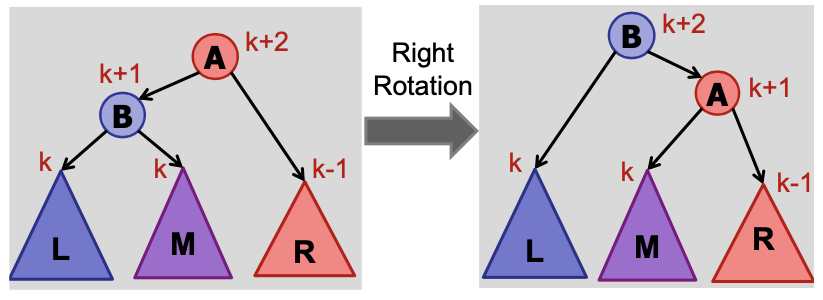
\includegraphics[width=0.85\linewidth]{cs2040s-rebalance-case-1.png}}
    
[case 2] B is  \textbf{left-heavy: right-rotate}
    \centerline{$h(L) = h(M) + 1, \quad h(R) = h(M)$}
    \centerline{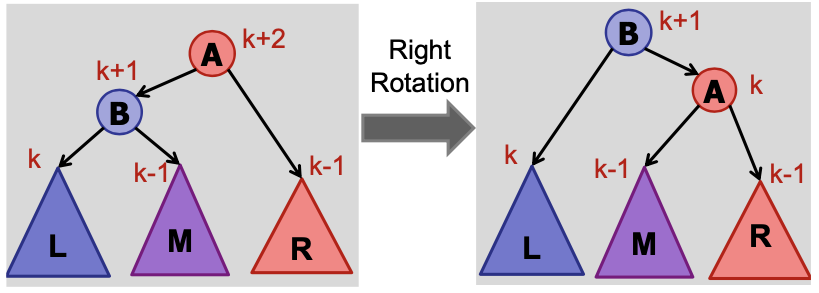
\includegraphics[width=0.85\linewidth]{cs2040s-rebalance-case-2.png}}

%\columnbreak 

[case 3] B is  \textbf{right-heavy: left-rotate(v.left), right-rotate(v)}
    \centerline{$h(L) = h(M) - 1, \quad h(R) = h(L)$}
    \centerline{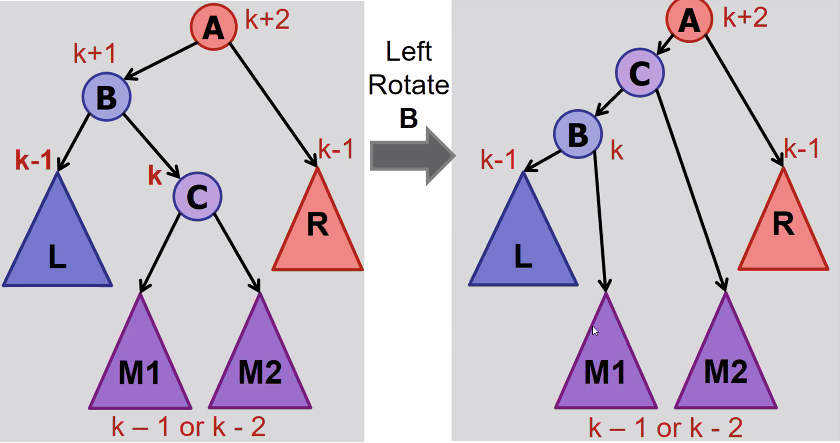
\includegraphics[width=0.5\linewidth]{cs2040s-rebalance-case-3-1.png}}
    \centerline{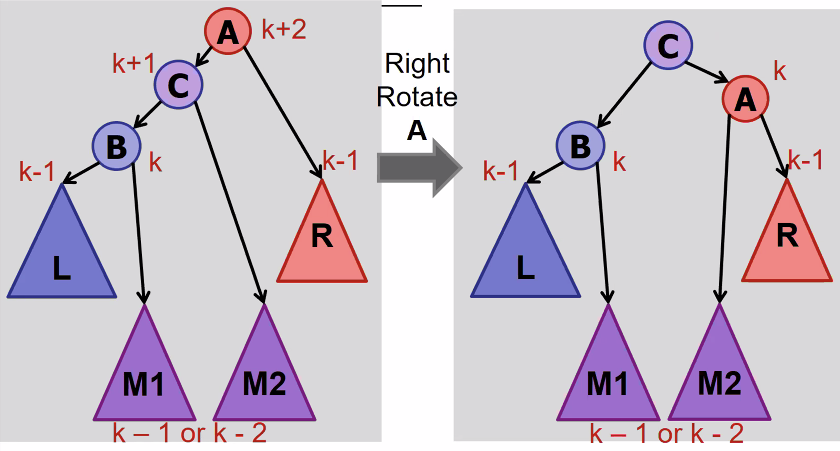
\includegraphics[width=0.5\linewidth]{cs2040s-rebalance-case-3-2.png}}

\subsection{updating nodes after rotation}
\begin{center}
    Order Statistics: weights
    \centerline{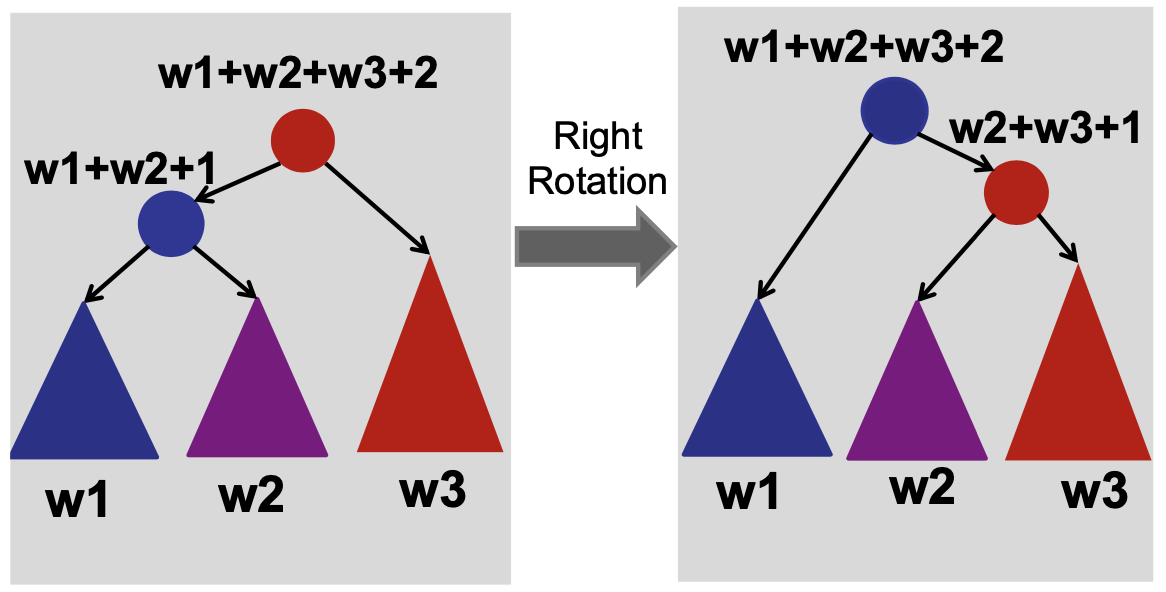
\includegraphics[width=0.5\linewidth]{cs2040s-rotate-weights.png}}
    
    Interval Trees: max endpoint in subtree
    \\* 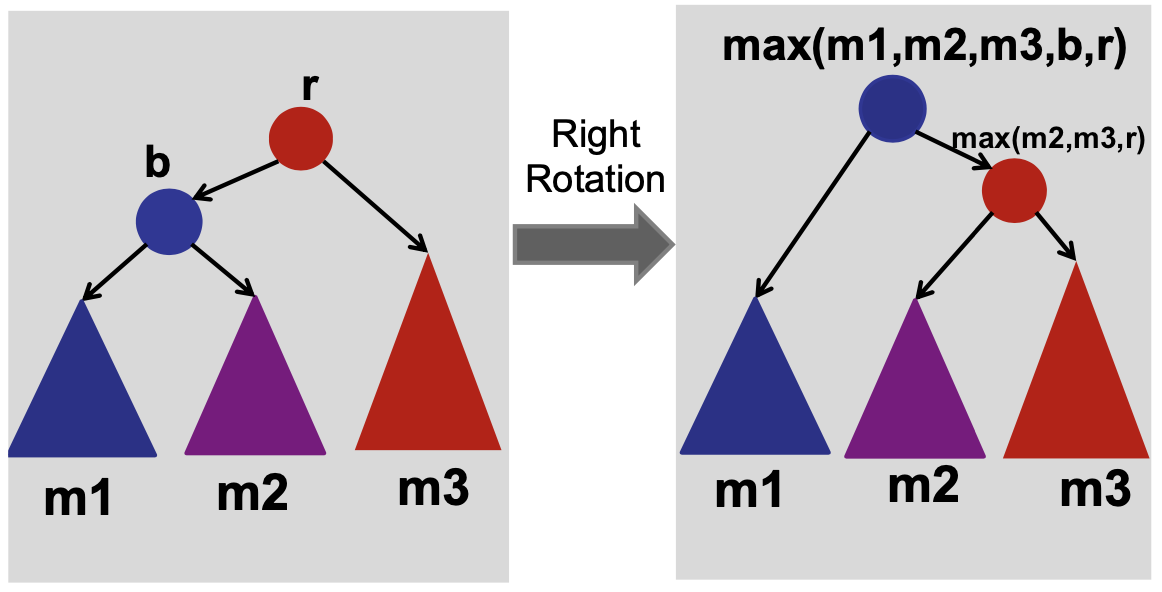
\includegraphics[width=0.5\linewidth]{cs2040s-rotate-max.png}
\end{center}

\textbf{AVL Tree Rotations:}
\begin{tightcenter}
    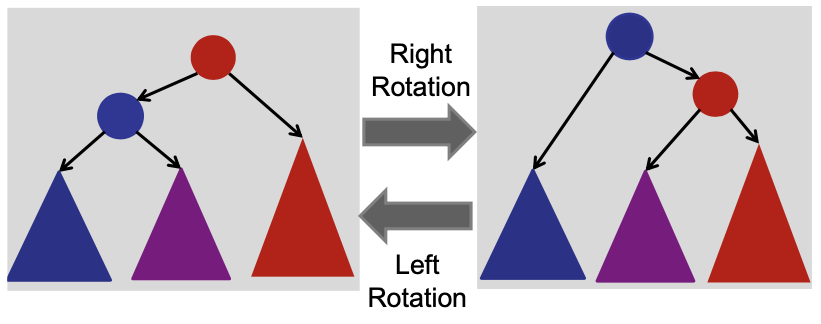
\includegraphics[width=0.8\linewidth]{cs2040s-tree-rotation.png}
\end{tightcenter}
\begin{itemize}
    \item insertion: max. 2 rotations
    \item deletion: recurse all the way up
    \item rotations can create every possible tree shape.
\end{itemize}

\subsection{Trie}
\begin{itemize}
    \item \code{search, insert} - $O(L)$ (for string of length $L$)
    \item space: $O($size of text $\cdot$ overhead$)$
\end{itemize}

\subsection{interval trees}
\begin{itemize}
    \item \code{search(key)} $\Then O(\log n)$
    \begin{itemize}
        \item if value is in root interval, return
        \item if value > max(left subtree), recurse right
        \item else recurse left (go left only when can't go right)
    \end{itemize}
    \item all-overlaps $\Then O(k \log n)$ for $k$ overlapping intervals
\end{itemize}

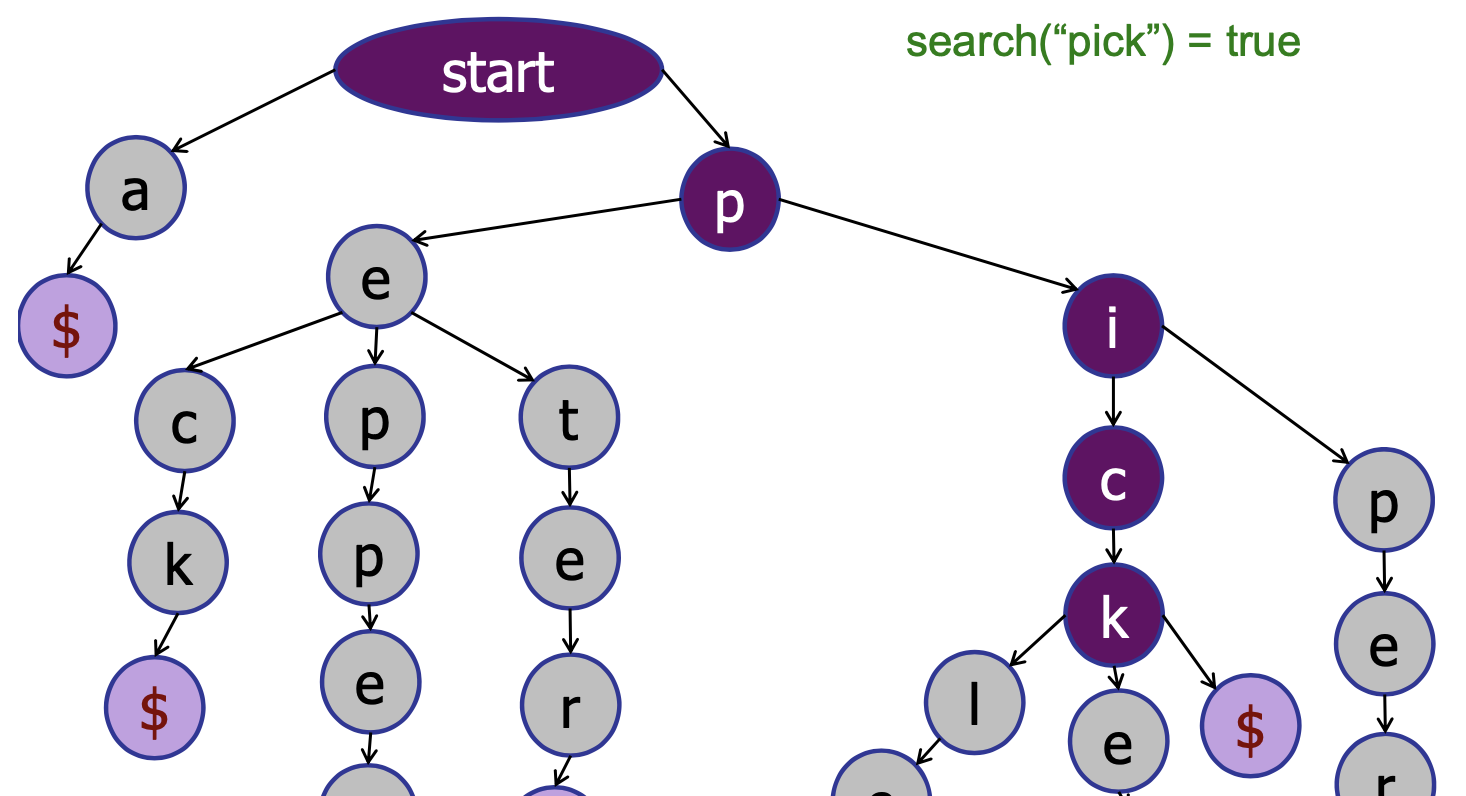
\includegraphics[width=0.5\linewidth]{cs2040s-trie.png}
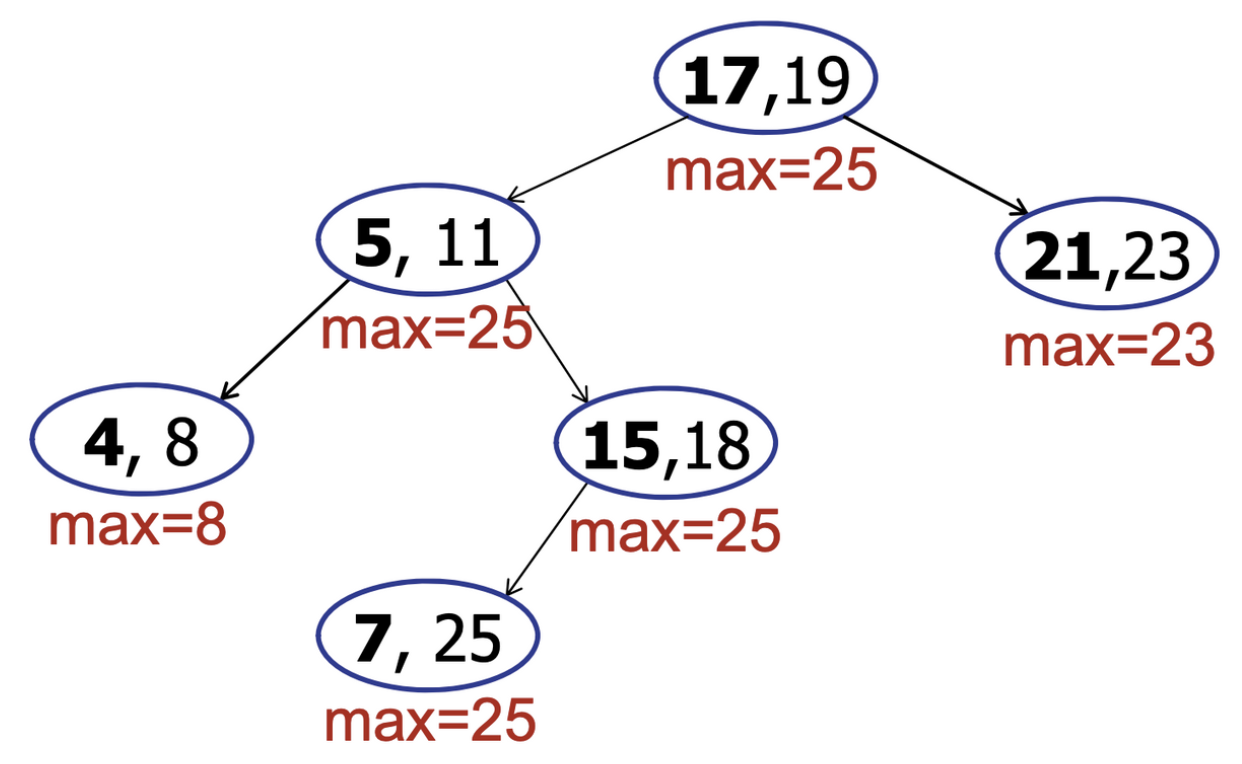
\includegraphics[width=0.45\linewidth]{cs2040s-interval-tree.png}

\subsection{orthogonal range searching (bBST)}
\begin{itemize}
    \item binary tree; leaves store points, internal nodes store max value in left subtree
    \item \code{buildTree(points[])} $\Then O(n \log n)$ \quad (space is $O(n)$)
    \item \code{query(low, hight)} $\Then O(k + \log n)$ for $k$ points
    \begin{itemize}
        \item \code{v=FindSplit()} $\Then O(\log n)$ - find node b/w low \& high
        \item \code{leftTraversal(v)} $\Then O(k)$ - either output all the right subtree and recurse left, or recurse right 
        \item \code{rightTraversal(v)} - symmetric
    \end{itemize}
    \item \code{insert(key), insert(key)} $\Then O(\log n)$ 
    \item \code{2D\_query()} $\Then O(\log^2n + k)$ \quad (space is $O(n \log n)$)
    \begin{itemize}
        \item build x-tree from x-coordinates; for each node, build a y-tree from y-coordinates of subtree
    \end{itemize}
    \item \code{2D\_buildTree(points[])} $\Then O(n \log n)$
\end{itemize}

\subsection{kd-Tree}
\begin{tightcenter}
    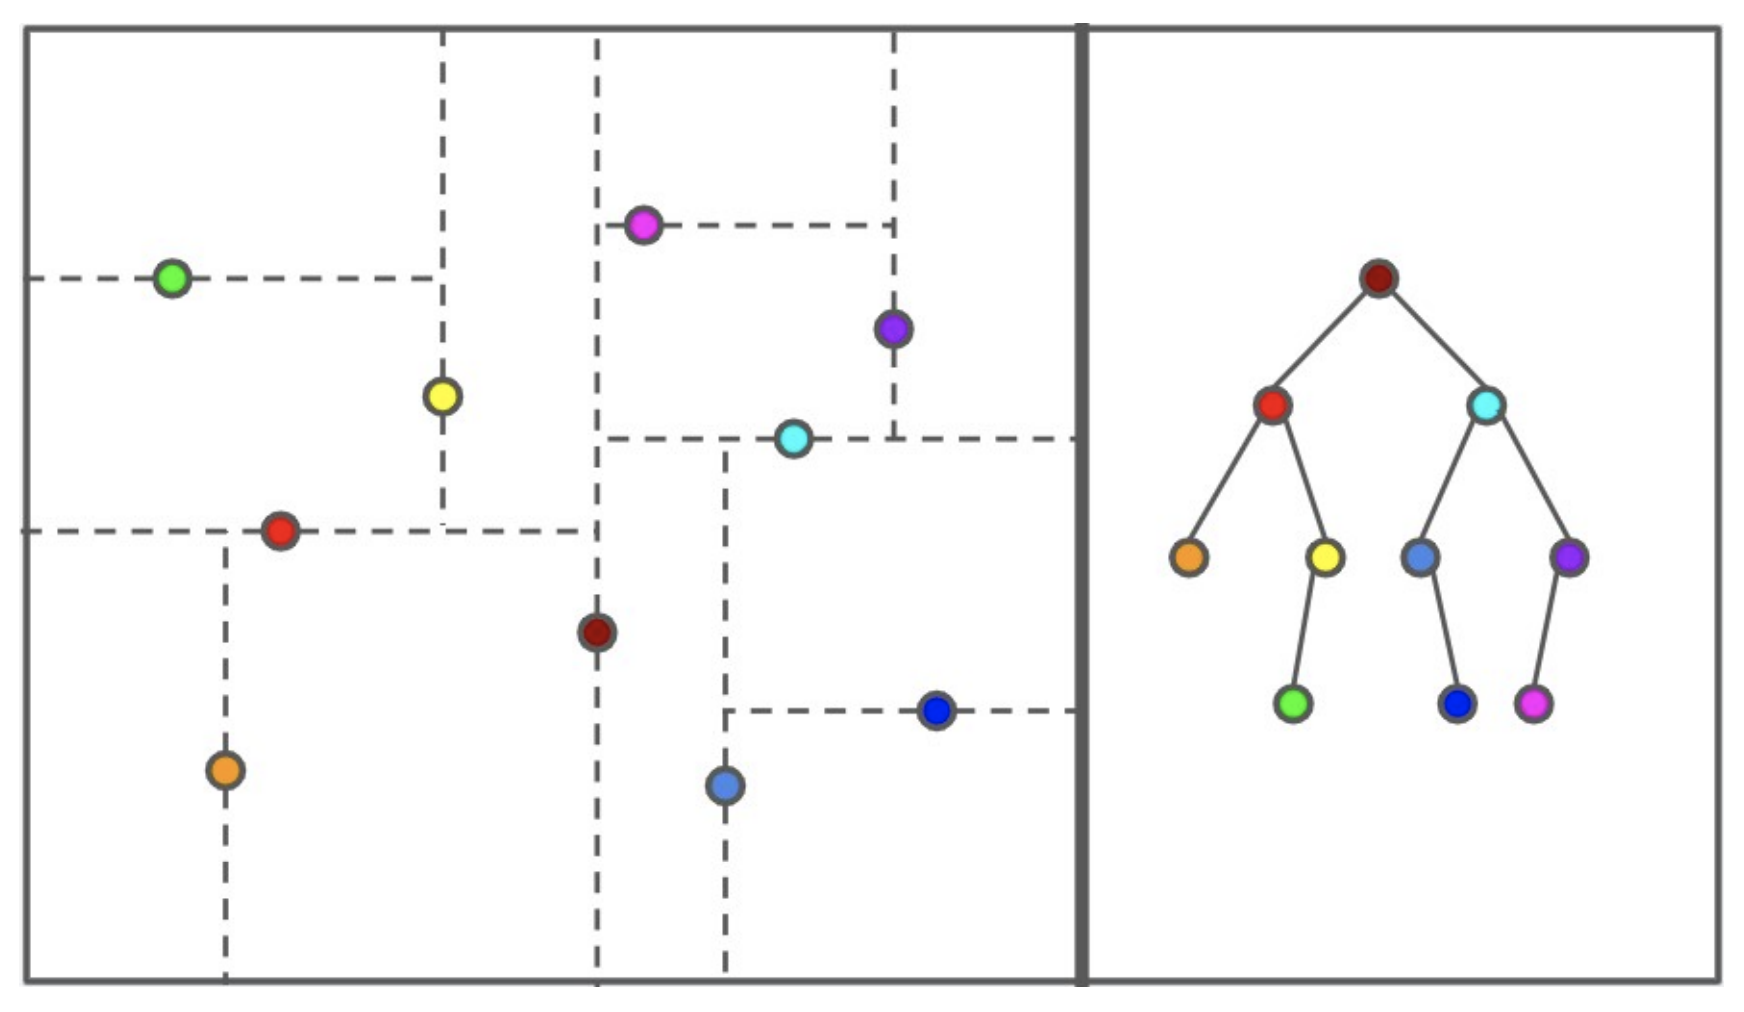
\includegraphics[width=0.4\linewidth]{cs2040s-kdtree.png}
\end{tightcenter}
\begin{itemize}
    \item stores geometric data (points in an $(x, y)$ plane)
    \item alternates splitting (partitioning) via $x$ and $y$ coordinates
    \item \code{construct(points[])} $\Then O(n \log n)$
    \item \code{search(point)} $\Then O(h)$
    \item \code{searchMin()} $\Then T(n) = 2T(\frac{n}{4}) + O(1) \Then O(\sqrt{n})$
\end{itemize}

\subsection{(a, b)-trees}
{\scriptsize{e.g. a (2, 4)-tree storing 18 keys}}
	\centerline{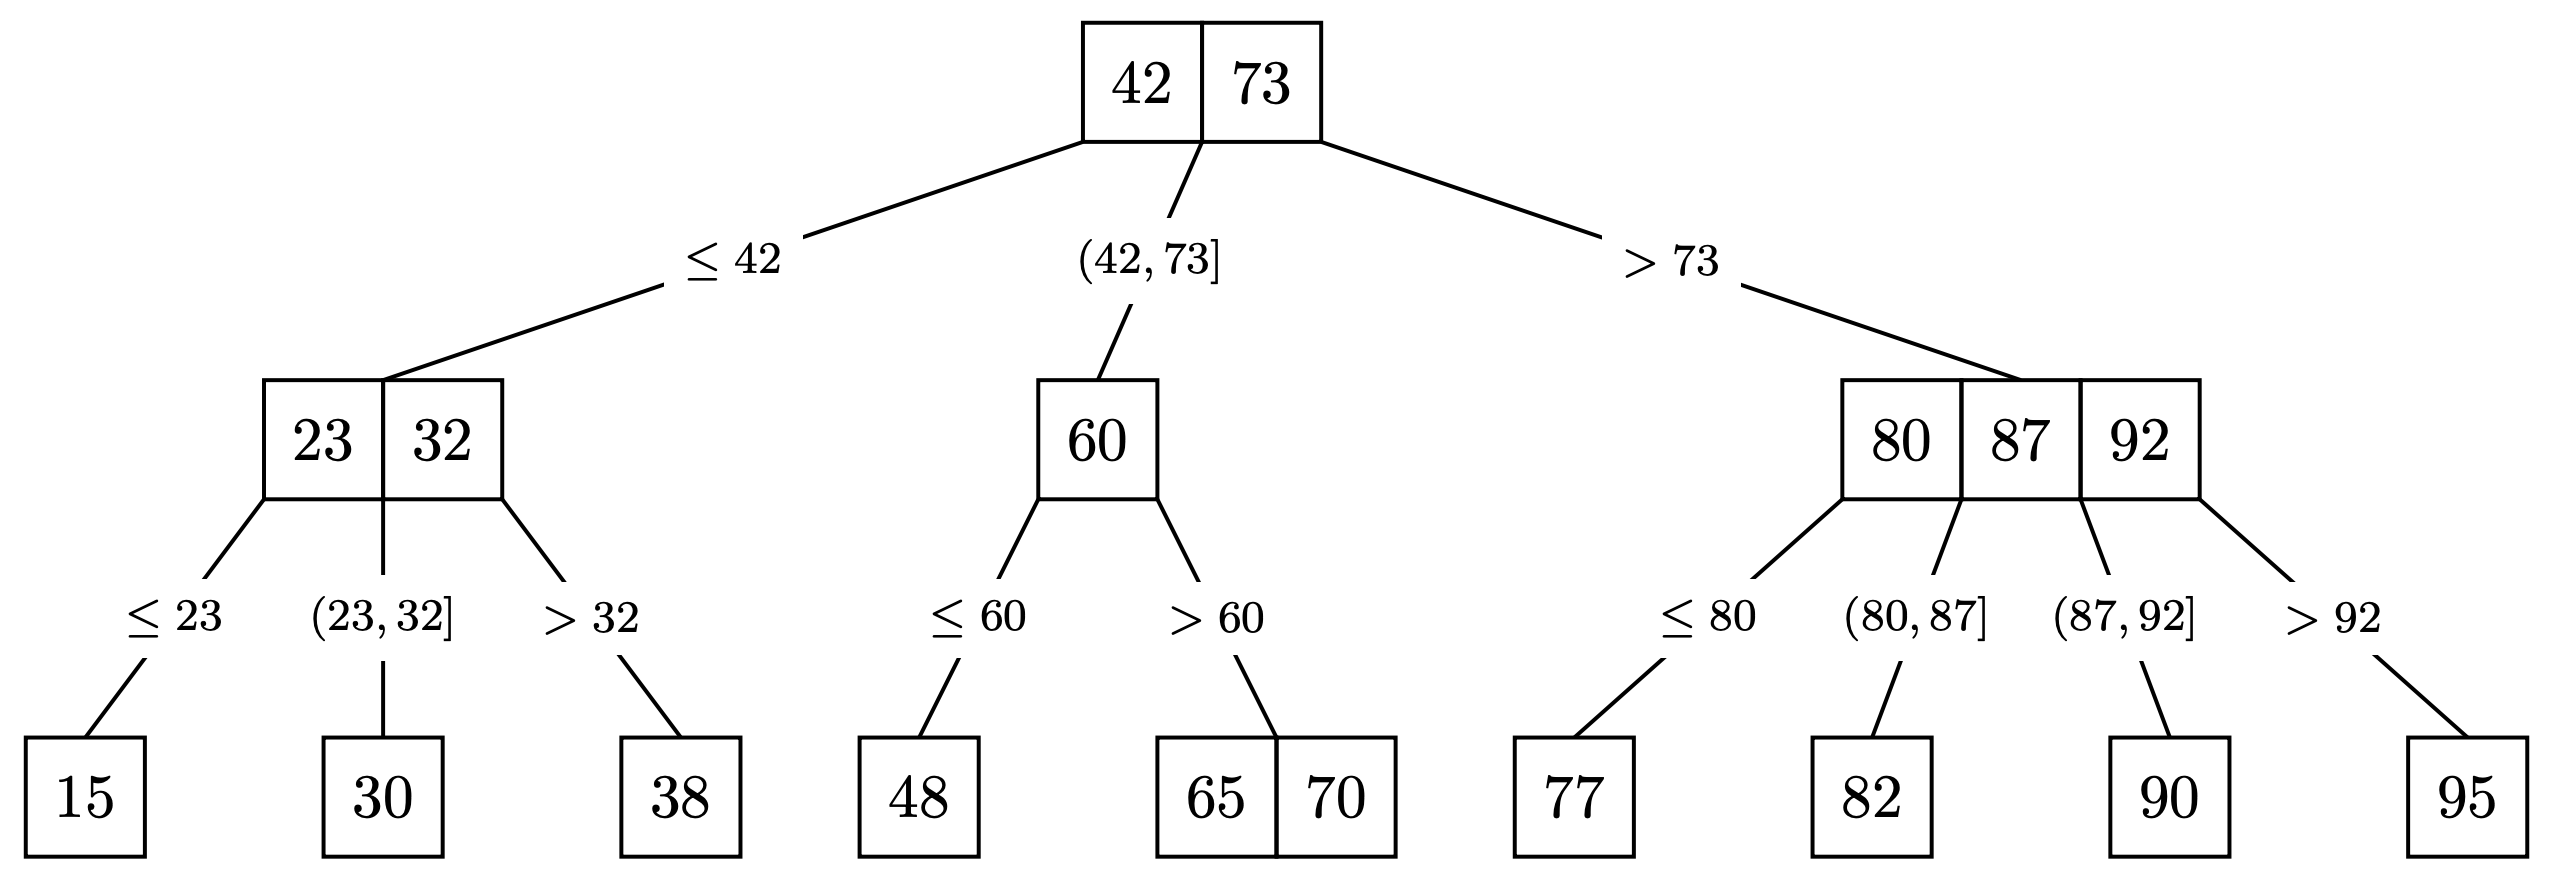
\includegraphics[width=0.7\linewidth]{cs2040s-ab-tree.png}}
\begin{itemize}
    \item \textbf{Rules:}
    \begin{enumerate}
        \item $(a, b)$-child policy where $2 \leq a \leq (b+1)/2$
        \begin{tabular}{|c|c|c|c|c|}
            \hline 
             & \multicolumn{2}{c|}{\# keys} & \multicolumn{2}{c|}{\# children}
            \\\hline
            node type & min & max & min & max
            \\\hline
            root & $1$ & $b-1$ & $2$ & $b$
            \\\hline
            internal & $a-1$ & $b-1$ & $a$ & $b$
            \\\hline
            leaf & $a-1$ & $b-1$ & $0$ & $0$
            \\\hline
        \end{tabular}
        \item an internal node has 1 more child than its number of keys
        \item all leaf nodes must be at the \textbf{same depth} from the root
    \end{enumerate}
    \item terminology (for a node $z$)
    \begin{itemize}
        \item key range - range of keys covered in subtree rooted at $z$
        \item keylist - list of keys within $z$
        \item treelist - list of $z$'s children
    \end{itemize}
    \item max height $= O(\log_an) + 1$
    \item min height $= O(\log_bn)$
    \item \code{search(key)} $\Then O(\log n)$ = $O(\log_2 b \cdot \log_a n)$ for binary search at each node
    \item \code{insert(key)} $\Then O(\log n)$
    \item \code{split()} a node with too many children
    \begin{enumerate}
        \item use median to split the keylist into 2 halves
        \item move median key to parent; re-connect remaining nodes
        \item (if the parent is now unbalanced, recurse upwards; if the root is reached, median key becomes the new root)
    \end{enumerate}
    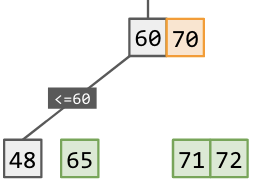
\includegraphics[width=0.4\linewidth]{cs2040s-abtree-split-1.png}
    $\Then$
    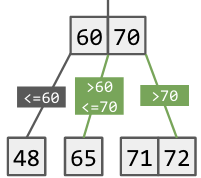
\includegraphics[width=0.3\linewidth]{cs2040s-abtree-split-2.png}
    \item \code{delete(key)} $\Then O(\log n)$
    \begin{itemize}
        \item if the node becomes empty, \code{merge(y, z)} - join it with its left sibling \& replace it with their parent
        \\* 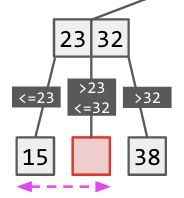
\includegraphics[width=0.25\linewidth]{cs2040s-abtree-delete-1.png}
        $\Then$
        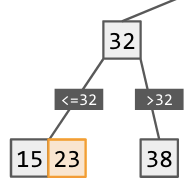
\includegraphics[width=0.3\linewidth]{cs2040s-abtree-delete-2.png}
        \item if the combined nodes exceed max size: \code{share(y, z)} = \code{merge(y, z)} then \code{split()}
    \end{itemize}
\end{itemize}

\subsection{B-Tree}
\begin{itemize}
    \item $(B, 2B)$-trees $\Then (a, b)$-tree where $a=B, b=2B$ 
    \item possible augmentation: use a linkedList to connect between each level
\end{itemize}


\section{HEAPS}
\textbf{Heaps vs. AVL Trees as Priority Queues}: Same asymptotic cost for operations. Heaps faster real cost, simpler (no rotations), slightly better concurrency.
\begin{enumerate}
    \item \textbf{heap ordering} - priority[parent] $\geq$ priority[child]
    \item \textbf{complete binary tree} - every level (except last level) is full; all nodes as far left as possible
\end{enumerate}
\begin{itemize}
    \item \textbf{Supported Operations}: all $O($max height$) = O(\floor{\log n})$
    \begin{itemize}
        \item \code{insert}: insert as leaf, bubble up to fix ordering
        \item \code{increase/decreaseKey}: bubble up/down larger key
        \item \code{delete}: swap w bottomrightmost in subtree; bubble down
        \item \code{extractMax}: Extract root then \code{delete(root)}, bubble down swapped last node towards larger key
    \end{itemize}
    \item heap \textbf{as an array}:
    \begin{itemize}
        \item \code{left(x)} $= 2x + 1$, $\quad$ \code{right(x)} $= 2x + 2$
        \item \code{parent(x)} $= \floor{\frac{x-1}{2}}$
    \end{itemize}
    \item \textbf{HeapSort}: $\then O(n \log n)$ always
    \begin{itemize}
        \item unsorted arr to heap: $O(n)$ (bubble down, low to high)
        \item heap to sorted arr: $O(n \log n)$ (extractMax, swap to back)
    \end{itemize}
\end{itemize}

\section{UNION-FIND}
\begin{itemize}
    \item Disjoint-Set Data Structure
    \item \textbf{quick-find} - \code{int[] componentId}, flat trees
    \begin{itemize}
        \item $O(1)$ find - check if objects have the same componentId
        \item $O(n)$ union - enumerate all items in array to update id
    \end{itemize}
    \item \textbf{quick-union} - \code{int[] parent}, deeper trees
    \begin{itemize}
        \item $O(n)$ find - check for same root (common parent)
        \item $O(n)$ union - add as a subtree of the root
    \end{itemize}
    \item \textbf{weighted union} - \code{int[] parent}, \code{int[] size}
    \begin{itemize}
        \item $O(\log n)$ find - check for same root (common parent)
        \item $O(\log n)$ union - add as a smaller tree as subtree of root
    \end{itemize}
    \item \textbf{path compression} - set parent of each traversed node to the root - $O(\log n)$ find, $O(\log n)$ union
    \begin{itemize}
        \item a binomial tree remains a binomial tree
    \end{itemize}
    \item \textbf{weighted union + path compression} - for $m$ union/find operations on $n$ objects: $O(n + m\alpha (m, n))$
    \begin{itemize}
        \item $O(\alpha (m, n))$ find, $O(\alpha (m, n))$ union
    \end{itemize}
\end{itemize}

\section{PROBABILITY THEORY}
\begin{itemize}
    \item if an event occurs with probability $p$, the expected number of iterations needed for this event to occur is $\frac{1}{p}$.
    \item for \textbf{random variables}: expectation is always equal to the probability
    \item \textbf{linearity of expectation}: $E[A + B] = E[A] + E[B]$
\end{itemize}

\section{UNIFORMLY RANDOM PERMUTATION}
\begin{itemize}
    \item for an array of $n$ items, every of the $n!$ possible permutations are producible with probability of exactly $\frac{1}{n!}$
    \begin{itemize}
        \item the number of outcomes should distribute over each permutation uniformly. (i.e. $\frac{\text{\# of outcomes}}{\text{\# of permutations}} \in \mathbb{N}$)
    \end{itemize}
    \item probability of an item remaining in its initial position $= \frac{1}{n}$
    \item \textbf{KnuthShuffle} $\Then O(n)$ - for every element in array $A$, swap it with a random index in array $A$. 
\end{itemize}

  
\end{multicols}

% Dividing Line
\hrulefill \\

\begin{multicols}{3}
    \begin{tightcenter}
        $
        \begin{array}{| c | c | c | c | c | c |}
            \hline\textbf{sort} & \textbf{best} & \textbf{average} & \textbf{worst} & \textbf{stable?} & \textbf{memory}
    
            \\\hline\text{bubble} & \Omega(n) & O(n^2) & O(n^2) & \checkmark & O(1)
            
            \\\hline\text{selection} & \Omega(n^2) & O(n^2) & O(n^2) & \times & O(1)
            
            \\\hline\text{insertion} & \Omega(n) & O(n^2) & O(n^2) & \checkmark & O(1)
            
            \\\hline\text{merge} & \Omega(n\log n) & O(n\log n) & O(n\log n) & \checkmark & O(n)
            
            \\\hline\text{quick} & \Omega(n\log n) & O(n\log n) & O(n^2) & \times & O(1)
            
            \\\hline\text{heap} & \Omega(n\log n) & O(n\log n) & O(n\log n) & \times & O(n)
            \\\hline
        \end{array} 
        $\
        \begin{tabular}{| c | c |}
            \multicolumn{2}{c}{sorting invariants}
            \\\hline\textbf{sort} & \textbf{invariant} (after $k$ iterations)
            \\\hline bubble & largest $k$ elements are sorted
            \\\hline selection & smallest $k$ elements are sorted
            \\\hline insertion & first $k$ slots are sorted
            \\\hline merge & given subarray is sorted
            \\\hline quick & partition is in the right position
            \\\hline
        \end{tabular} \begin{tabular}{| c | c |}
            \multicolumn{2}{c}{searching}\\\hline
            \textbf{search} & \textbf{average} \\\hline
            linear & $O(n)$ \\\hline
            binary & $O(\log n)$ \\\hline
            quickSelect & $O(n)$ \\\hline
            interval & $O(\log n)$ \\\hline
            all-overlaps & $O(k\log n)$ \\\hline
            1D range & $O(k + \log n)$ \\\hline
            2D range & $O(k + \log^2 n)$ \\\hline
        \end{tabular}
        
        data structures assuming $O(1)$ comparison cost
        \\* \begin{tabular}{| c | c | c |}\hline
            \textbf{data structure} & \textbf{search} & \textbf{insert}\\\hline
            sorted array & $O(\log n)$ & $O(n)$ \\\hline
            unsorted array & $O(n)$ & $O(1)$ \\\hline
            linked list & $O(n)$ & $O(1)$ \\\hline
            tree (kd/(a, b)/binary) & $O(\log n)$ or $O(h)$ & $O(\log n)$ or $O(h)$ \\\hline
            trie & $O(L)$ & $O(L)$ \\\hline
            dictionary & $O(\log n)$ & $O(\log n)$ \\\hline
            symbol table & $O(1)$ & $O(1)$ \\\hline
            chaining & $O(n)$ & $O(1)$ \\\hline
            open addressing & $\frac{1}{1-\alpha} = O(1)$ & $O(1)$ \\\hline
        \end{tabular}

        \ 
        \\ orders of growth
        \\* $1 < \log n < \sqrt{n} < n < n \log n < n^2 < n^3 < 2^n < 2^{2n}$
        \\* $\log_a n < n^a < a^n < n! < n^n$

        orders of growth
        \begin{align*}
            T(n) &= 2T(\frac{n}{2}) + O(n) &\Rightarrow O(n \log n)
            \\ T(n) &= T(\frac{n}{2}) + O(n) &\Rightarrow O(n)
            \\ T(n) &= 2T(\frac{n}{2}) + O(1) &\Rightarrow O(n)
            \\ T(n) &= T(\frac{n}{2}) + O(1) &\Rightarrow O(\log n)
            \\ T(n) &= 2T(n - 1) + O(1) &\Rightarrow O(2^n)
            \\ T(n) &= 2T(\frac{n}{2}) + O(n \log n) &\Rightarrow O(n(\log n)^2)
            \\ T(n) &= 2T(\frac{n}{4}) + O(1) &\Rightarrow O(\sqrt{n})
            \\ T(n) &= T(n - c) + O(n) &\Rightarrow O(n^2)
        \end{align*}
    \end{tightcenter}
\end{multicols}

\end{document}